\documentclass[12pt]{article}
\usepackage[a4paper, total={5.5in, 9in}]{geometry}
\usepackage{amsmath}
\usepackage{amsfonts}
\usepackage{graphicx}
\usepackage{pgfplots} % Para crear gráficos
\pgfplotsset{compat=1.18} % Para evitar warnings de compatibilidad
\usepackage{enumitem}

\title{College Algebra Worksheet 3.2}
\author{PCL Learning Center}
\date{}

\begin{document}
\maketitle

\begin{center}
    \textit{note: No graphing calculators or electronic devices may be used on this worksheet.}    
\end{center}

\section*{Problem Set 1\\Difficulty level: Normal}
\subsection*{Problem 1}
Find the domain and range of the relation
\[\{(11,13),(\star, \oplus),(18,0),(-1,-16),(-5,-1)\}\]

\subsection*{Problem 2}
Find the domain of the following function.
\[f(x)=\sqrt{2x-40}\]

\subsection*{Problem 3}
Find the domain of the function.
\[\{(1,-11),(-10,-4),(-8,11),(4,-2)\}\]

\subsection*{Problem 4}
Find the domain of the following function.
\[h(x)=4x^3+2x+1\]

\subsection*{Problem 5}
Find the domain of the following function.
\[f(x)=\dfrac{1}{\sqrt{17x-34}}\]

\subsection*{Problem 6}
Find the domain of the following function.
\[f(x)=\dfrac{1}{(x-5)(6-x)}\]

\subsection*{Problem 7}
When describing sets of numbers using interval notation, when do you use a parenthesis and when do you use a bracket?

\subsection*{Problem 8}
Find the domain and range from the graph. Write them in interval notation.

\begin{figure}[!ht]
    \centering
    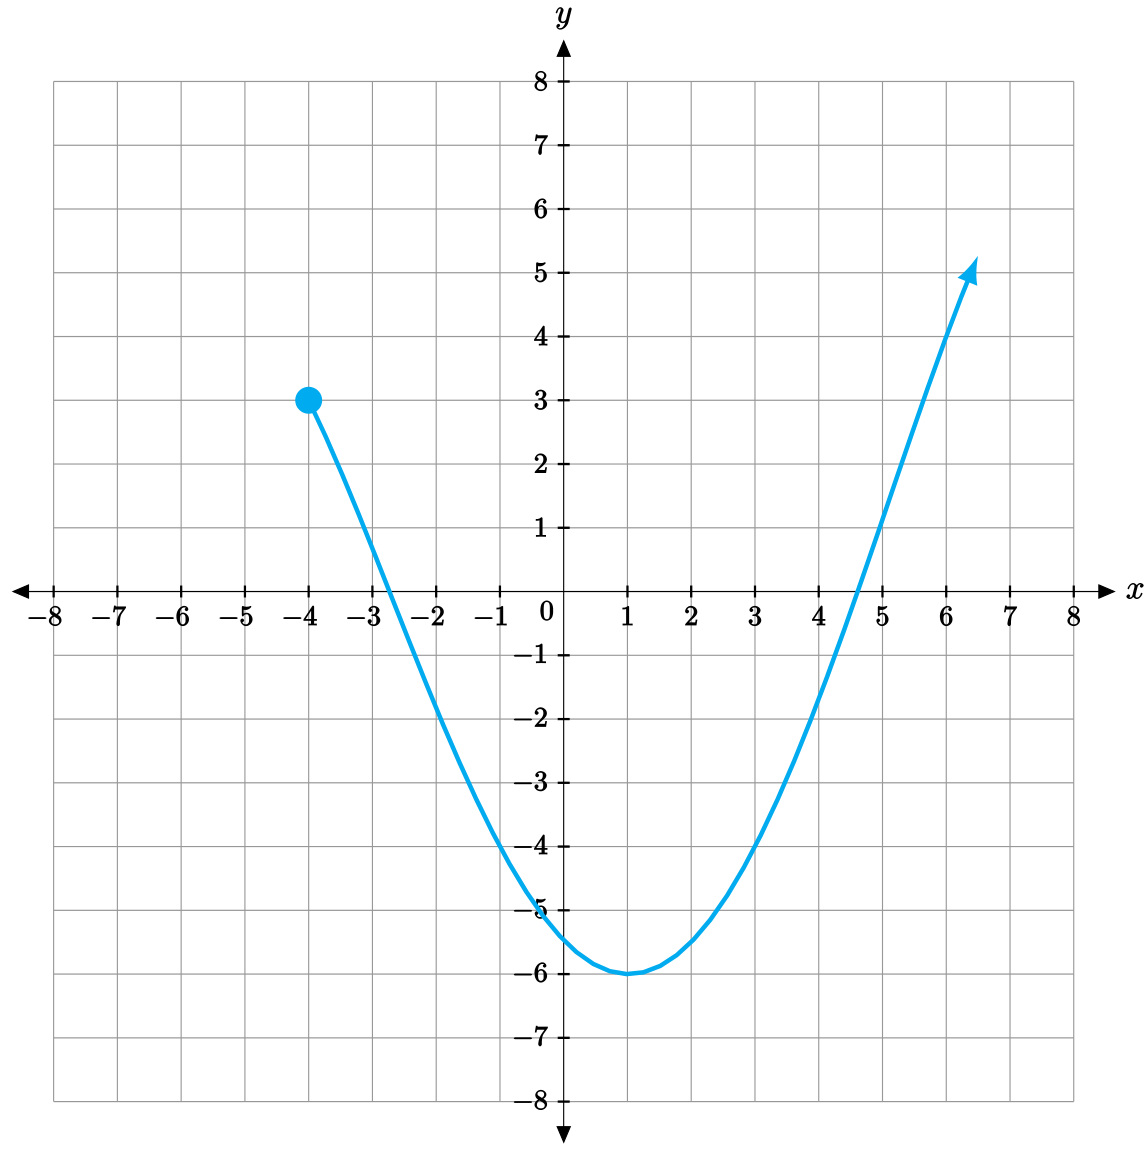
\includegraphics[width=\textwidth]{1.png}
\end{figure}



\subsection*{Problem 9}
Find the domain and range from the graph. Write them in interval notation.
\begin{figure}[!ht]
    \centering
    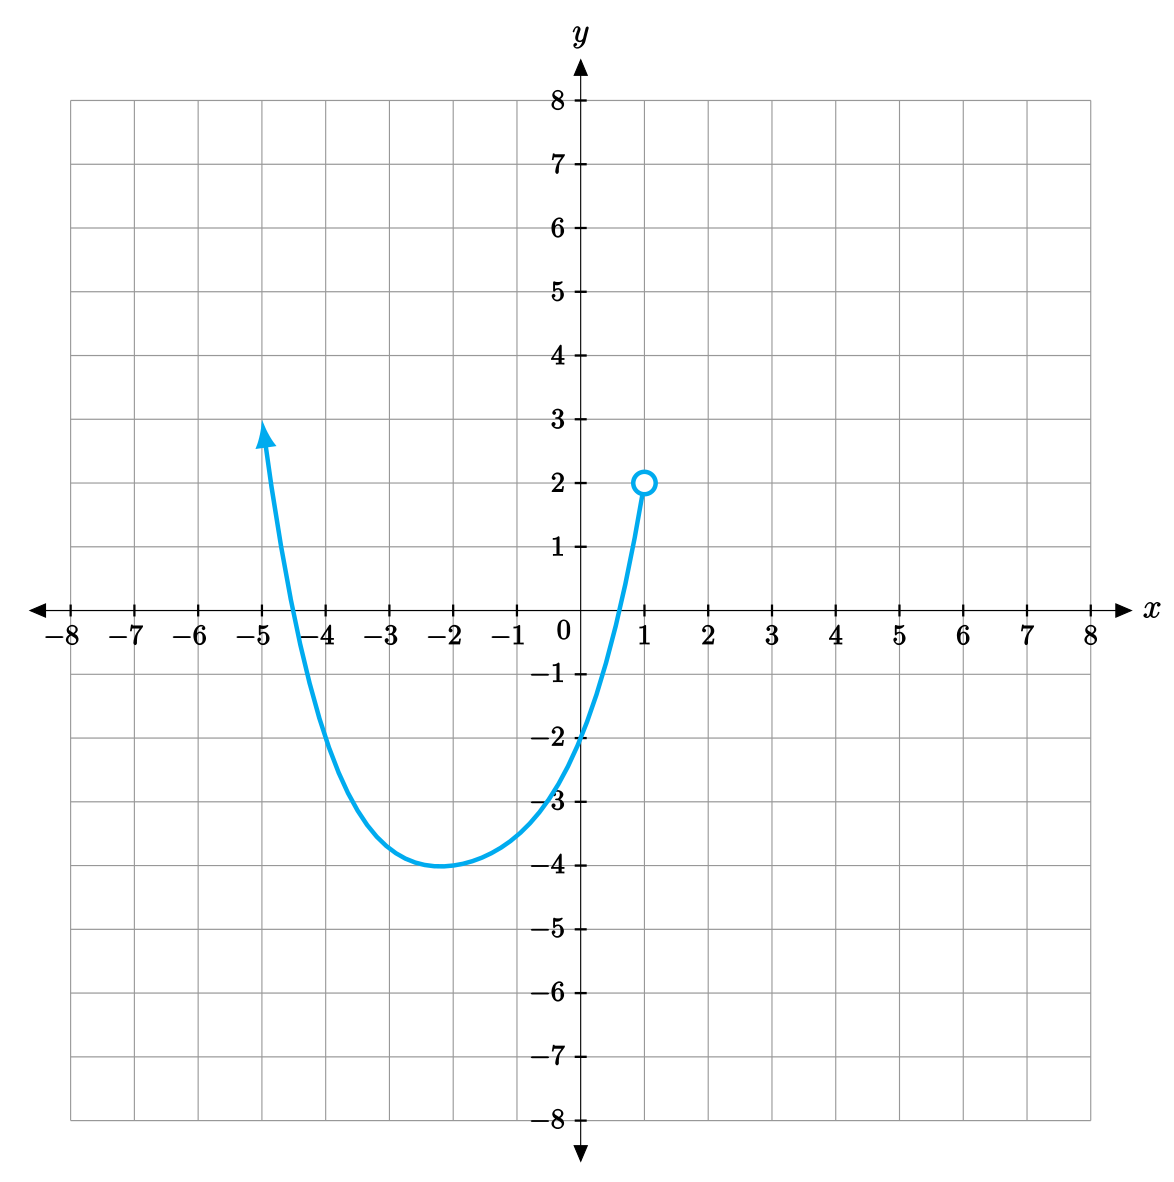
\includegraphics[width=0.7\linewidth]{2.png}
\end{figure}


\section*{Problem Set 2\\Difficulty level: Hard}
\subsection*{Problem 1}
Find the domain of the following function.
\[f(x)=\dfrac{2x^3-250}{x^2-2x-15}\]

\subsection*{Problem 2}
Graph the function, \(h(x)\), and find its domain and range.
\[h(x)=\sqrt{x^2+4}\]

\subsection*{Problem 3}
Explain why the domain of \(f(x)=\sqrt[3]{x}\) is different from the domain of \(f(x)=\sqrt{x}\)

\newpage
\section*{Solutions to Set 1}
\subsection*{Problem 1}
domain: \(\{\star,-5,-1,11,18\}\), range: \(\{\oplus,-16,-1,0,13\}\)\\
\textit{note: the order (position) of \(\star\) does not matter in the domain, since it is not a number, and similarly for the range for \(\oplus\).}
\subsection*{Problem 2}
domain: \([20,\infty)\)
\subsection*{Problem 3}
domain: \(\{-10,-8,1,4\}\)
\subsection*{Problem 4}
domain: \((-\infty,\infty)\)
\subsection*{Problem 5}
domain: \((2,\infty)\)
\subsection*{Problem 6}
domain: \((-\infty,5)\cup(5,6)\cup(6,\infty)\)
\subsection*{Problem 7}
We use parenthesis to mean that a number or object is not included, and otherwise for bracket.
\subsection*{Problem 8}
domain: \([-4,\infty)\), range: \([-6,\infty)\)
\subsection*{Problem 9}
domain: \((-\infty,1)\), range: \([-4,\infty)\)

\section*{Solutions to Set 2}
\subsection*{Problem 1}
Notice that
\[\dfrac{2x^3-250}{x^2-2x-15}=\dfrac{2x^3-250}{(x-5)(x+3)}=\dfrac{(x-5)(2x^2+10x+50)}{(x-5)(x+3)}\]
so the domain in interval notation is \((-\infty,-3)\cup (-3,\infty)\)
\subsection*{Problem 2}
domain: \((-\infty,\infty)\), range: \([2,\infty)\)
\subsection*{Problem 3}
The domain of \(f(x)=\sqrt{x}\) is \(x \geq 0\), because we can not take a square root of a negative number, but the domain of \(f(x)=\sqrt[3]{x}\) is all real numbers, since \(\sqrt[3]{x}\) can \textit{"accept"} positive and negative numbers.
\end{document}
